% PressureWTChar.tex

\tikzstyle{RectObject}=[rectangle,draw=blue,rounded corners,line width=0.5mm,
  minimum width=12em,minimum height=8em]
\tikzstyle{StallRectObject}=[rectangle,draw=blue,rounded corners,line width=0.5mm,
  minimum width=4em,minimum height=6.5em]
\tikzstyle{LabelObject}=[fill=white,rectangle,rounded corners,line width=0.5mm,%
	align=center]
\tikzstyle{ArrowObject}=[red,line width=1.0mm, -latex]

\resizebox{!}{0.45\textwidth}{
	\begin{tikzpicture}
		\node[anchor=south west,inner sep=0] (image) at (0,0)%
			{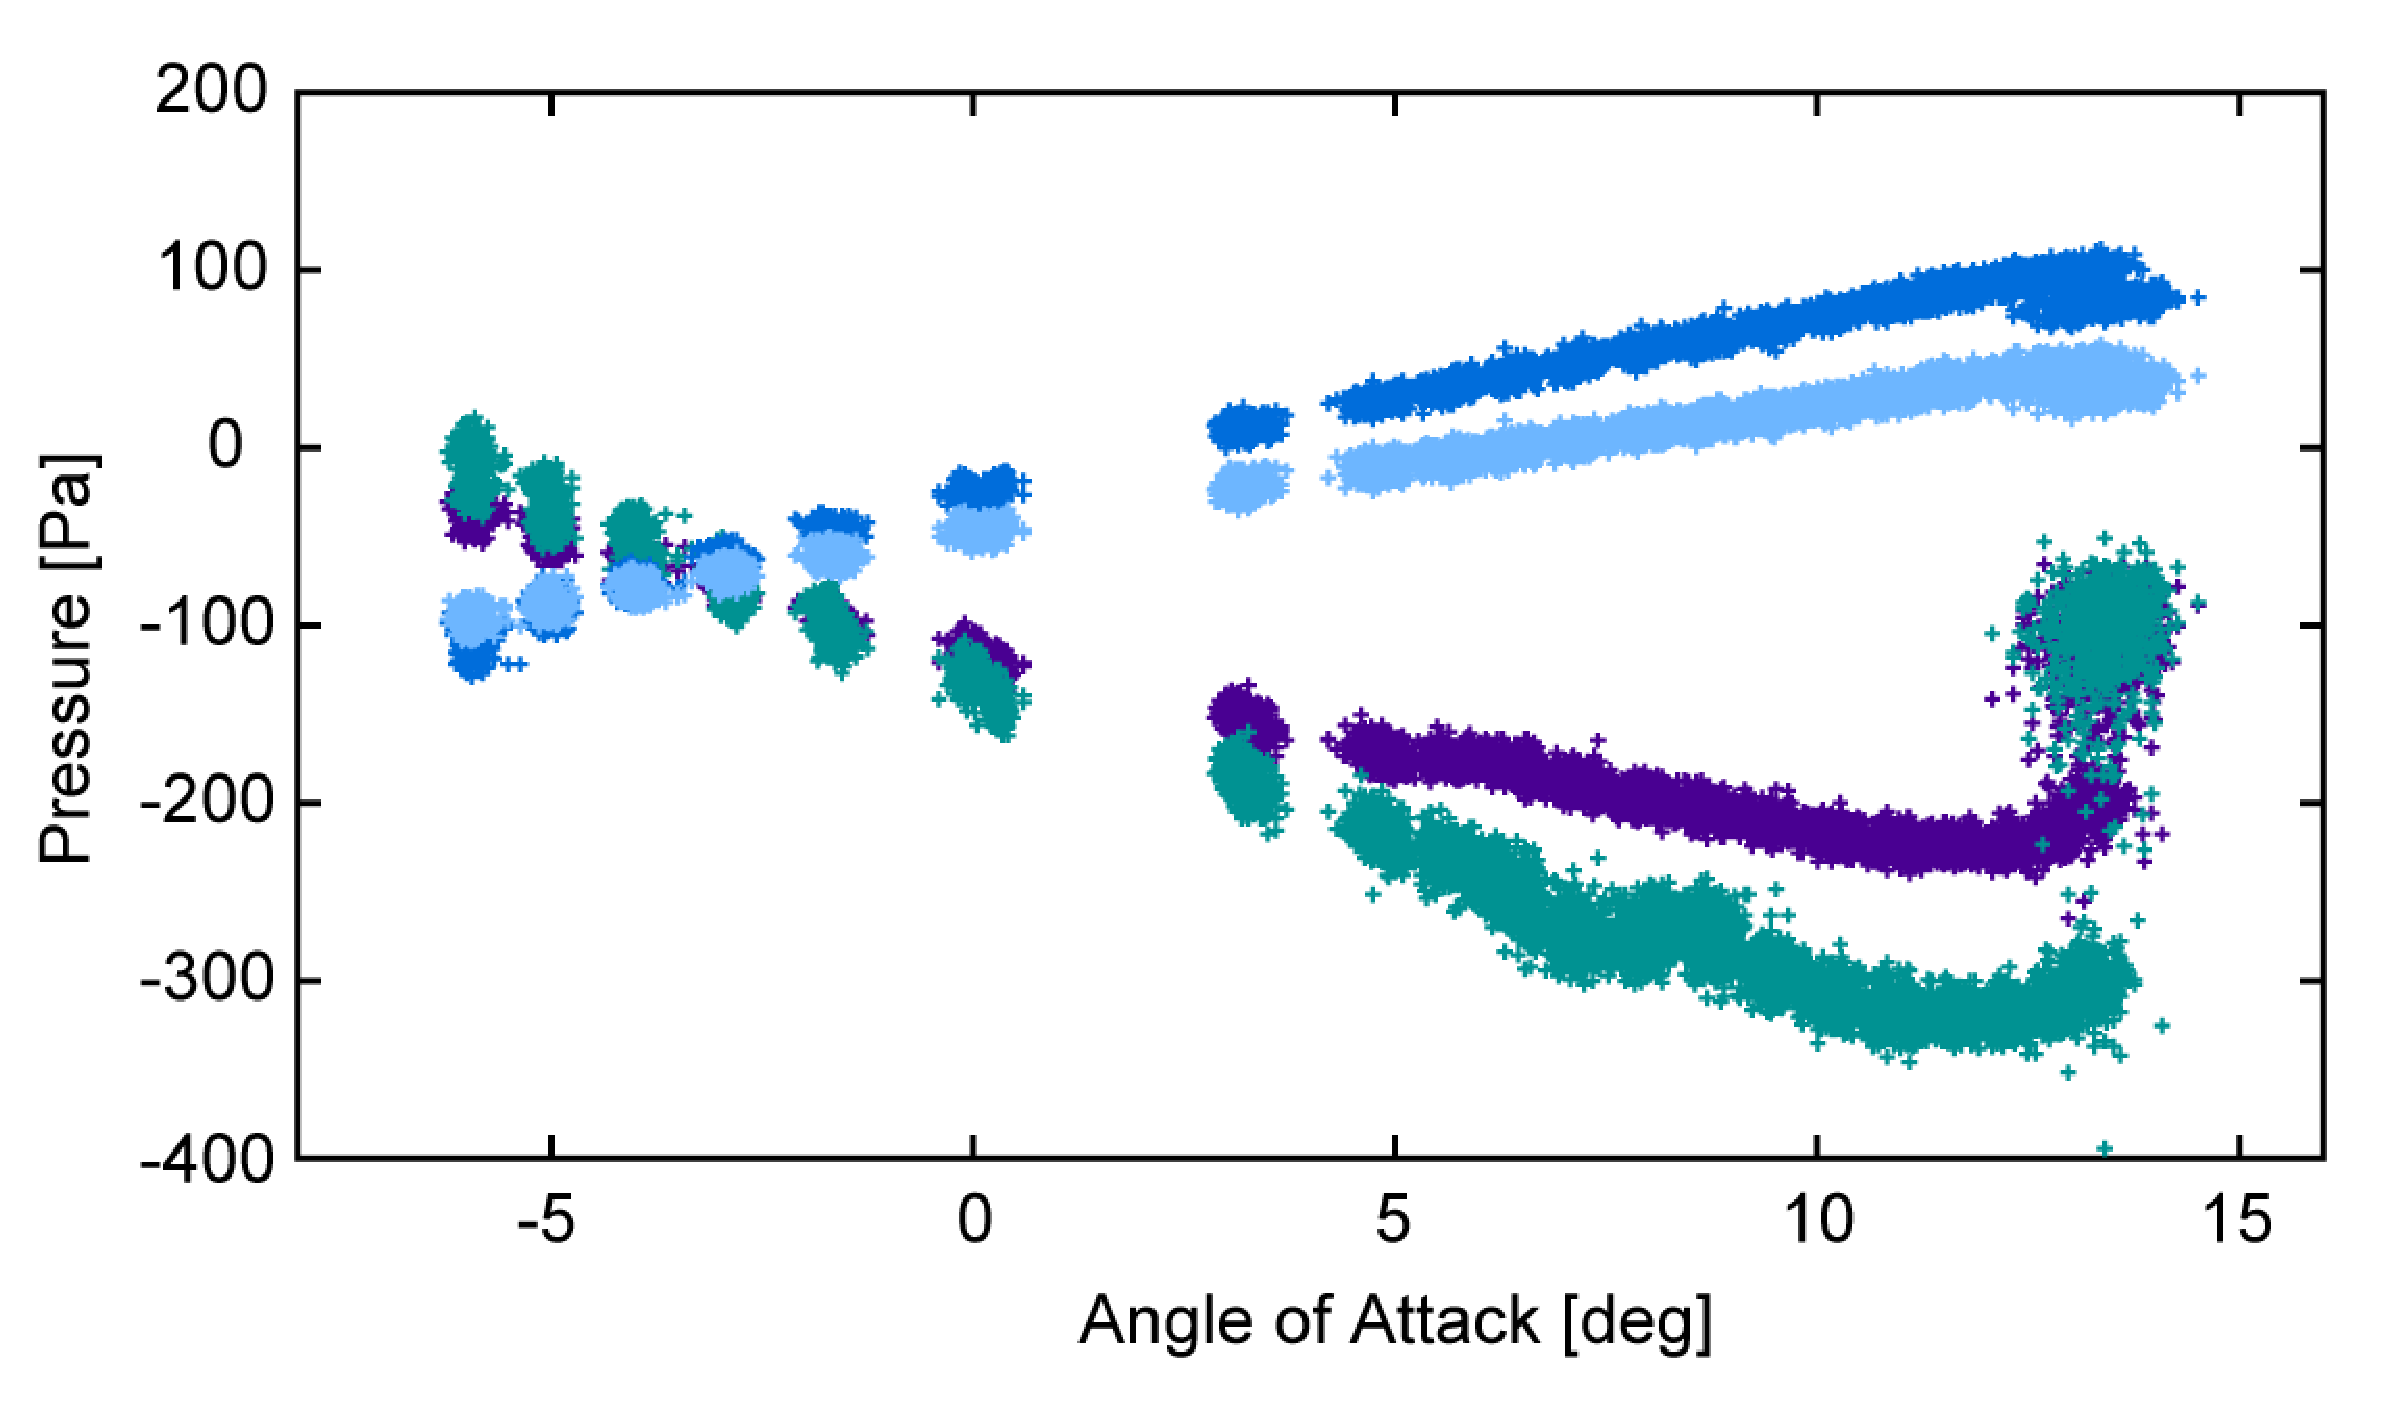
\includegraphics[width=\textwidth]{Flow-pressure-vs-AoA-no-lines.eps}};
		% Define scope with 'image' dimensions as reference
		\begin{scope}[x={(image.south east)},y={(image.north west)}]
			%\draw[help lines,xstep=.05,ystep=.05] (0,0) grid (1,1);
			%\foreach \x in {0,1,...,9} { \node [anchor=north] at (\x/10,0) {0.\x}; }
			%\foreach \y in {0,1,...,9} { \node [anchor=east] at (0,\y/10) {0.\y}; }
			
			% Aircraft diagram
			\node[anchor=south west,inner sep=0] (AircraftDiagram) at (0.15,0.80)%
			  {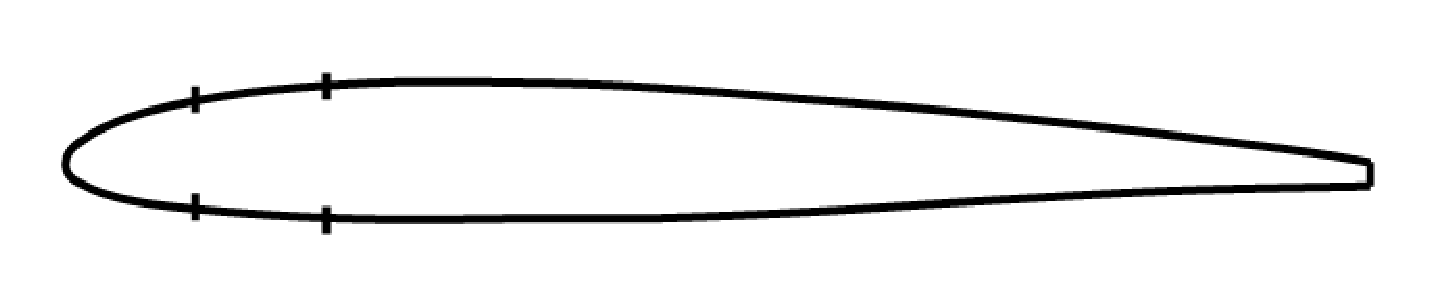
\includegraphics[width=0.5\textwidth]{Flow-wing-outline-no-label.eps}};
			  % Pressure sensors on aircraft
			  \draw(AircraftDiagram) ++(-0.140, 0.035) node[mark size=2pt,color=violet] (PS1) {\pgfuseplotmark{*}};
			  \draw(AircraftDiagram) ++(-0.185, 0.025) node[mark size=2pt,color=black!50!green]  (PS2) {\pgfuseplotmark{*}};
			  \draw(AircraftDiagram) ++(-0.185,-0.040) node[mark size=2pt,color=blue]   (PS4) {\pgfuseplotmark{*}};
				\draw(AircraftDiagram) ++(-0.140,-0.048) node[mark size=2pt,color=cyan]   (PS3) {\pgfuseplotmark{*}};
			
			\only<5>{
			  % Linear Pressure with AoA
			  \draw(0.45,0.55) node[RectObject] (LinPressure) {};
			  % Linear Pressure with AoA label
			  \draw(0.85,0.50) node[LabelObject] (LinPressure_Label) {Linear Pressure\\With AoA};
			}
			\only<6>{
			  % Pressure Stall Markers
			  \draw(0.85,0.425) node[StallRectObject] (PressureStall) {};
			  % Pressure Stall Markers label
			  \draw(0.30,0.45) node[LabelObject] (PressureStall_Label)
				  {Large increase\\in variance\\ during stall};
			  % Pressure Stall Markers arrow
			  \draw[ArrowObject] (PressureStall_Label.east) -- (PressureStall.west);
			}
			
		\end{scope}
  \end{tikzpicture}
}